Bei variierender Trainingsdauer auf dem Source-Datensatz zeigt sich, dass die Leistungsfähigkeit des Netzwerks auf dem Target-Datensatz 
unterschiedlich ausfällt. Da der optimale Zeitpunkt für den Einsatz von TF ohnehin ermittelt werden muss, wird im 
Folgenden das CMP-Netzwerk verwendet, wobei nach jedem Layer TF angewandt wird. Die daraus resultierenden Ergebnisse sind in Abbildung 
\ref{fig:layertf} dargestellt.

\begin{figure}[htpb]
    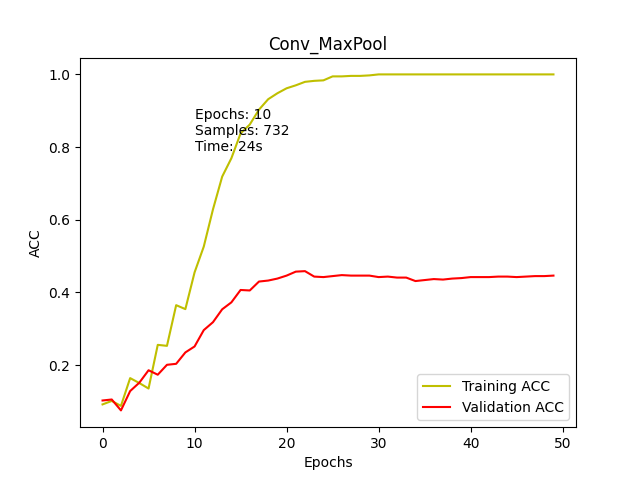
\includegraphics[height=5cm]{../../Plots/ba_plots/convmaxpool/wotr.png}
    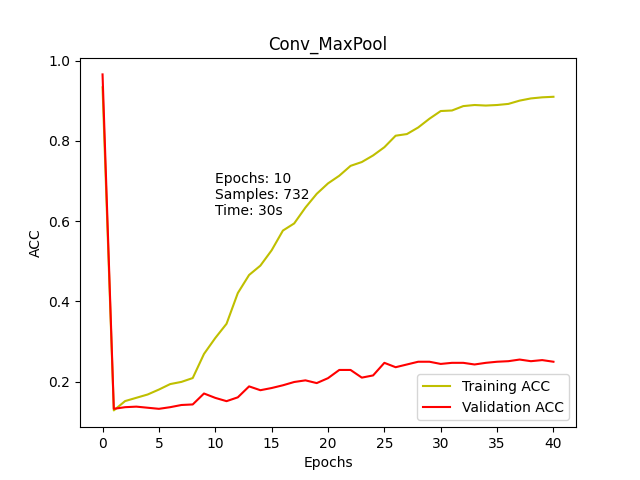
\includegraphics[height=5cm]{../../Plots/ba_plots/convmaxpool/epochTFtr.png}
    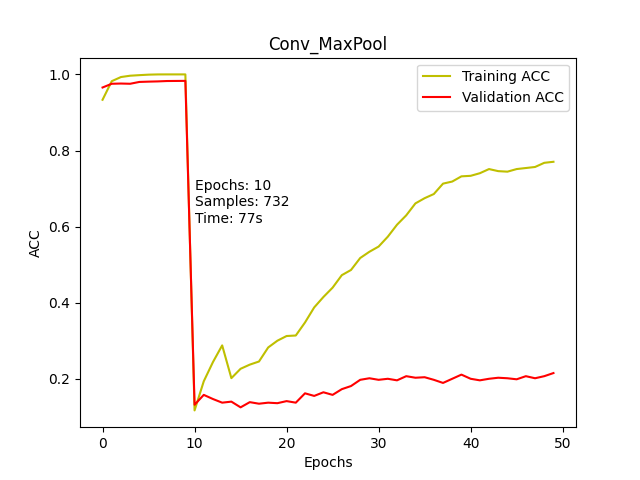
\includegraphics[height=5cm]{../../Plots/ba_plots/convmaxpool/1TFtr.png}
    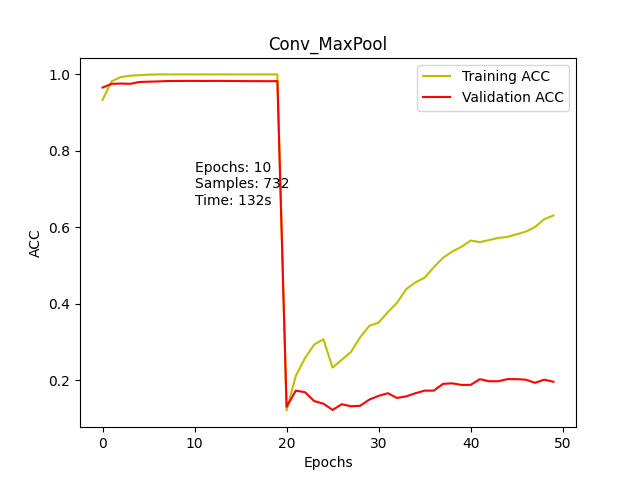
\includegraphics[height=5cm]{../../Plots/ba_plots/convmaxpool/2TFtr.png}
    % 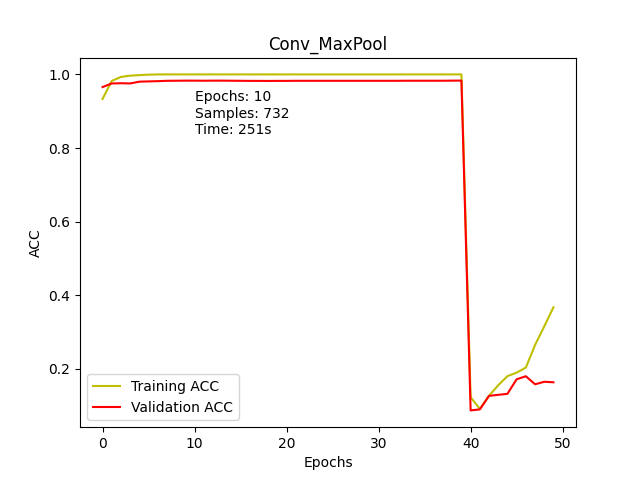
\includegraphics[height=5cm]{../../Plots/ba_plots/convmaxpool/4TFtr.png}
    \caption{\label{fig:layertf} 
    \small{In der Abbildung sind von links oben nach rechts unten die Plots folgender Tests dargestellt: CMP:732/10, CMP:TF0/732/10, 
    CMP:TF1/732/10 sowie CMP:TF2/732/10. Bei allen dargestellten Plots zeigt sich ein ähnliches Problem, nämlich eine zunehmende Diskrepanz 
    zwischen Trainings-Accuracy und Validierungs-Accuracy über den Trainingsverlauf hinweg.}}
\end{figure}

Es fällt auf, dass die beste Performanz ohne den Einsatz von TF erzielt wird. Bereits nach nur einer Trainings-Epoche im 
ersten Layer, das auf dem Source-Datensatz trainiert wird, ist ein deutlicher Einbruch der Accuracy zu beobachten. Dies legt nahe, dass TF im 
Kontext von Klassifikationsaufgaben mit Deep Cascade Netzwerken wenig sinnvoll ist. Das Trainingsset, das bei TF verwendet wird, erreicht nie 
annähernd die Leistungsbereiche, die ohne TF erzielt werden. 
Dabei nimmt die Accuracy auf den Trainingsdaten mit zunehmender Verzögerung des Einsatzes von TF kontinuierlich ab. 
Daraus lässt sich ableiten, dass bereits ein Overfitting auf den Source-Datensatz 
stattgefunden hat, welches das Lernen auf dem Target-Datensatz erheblich erschwert. Dieses Overfitting tritt dabei bereits nach einem einzigen 
Layer auf dem Source-Datensatz auf, wie die Grafik unten links in Abbildung \ref{fig:layertf} verdeutlicht. Darüber hinaus ist in allen 
dargestellten Plots erkennbar, dass das Overfitting auf das Trainingsset des Target-Datensatzes vorhanden ist, da die Trainings-Accuracy dort 
um etwa 60\% höher liegt als bei der Validierungs- und bei der Test-Accuracy.

Im Gegensatz dazu zeigt ein Regressionsnetzwerk, wie das Deep Cascade Netzwerk RegressionTwo, wie in Abbildung \ref{fig:regr2tf} dargestellt, 
kein schnelles Auftreten von Overfitting. Weder auf dem Source-Datensatz noch auf dem Target-Datensatz lässt sich ein entsprechendes Verhalten 
beobachten.

\begin{figure}[htpb]
    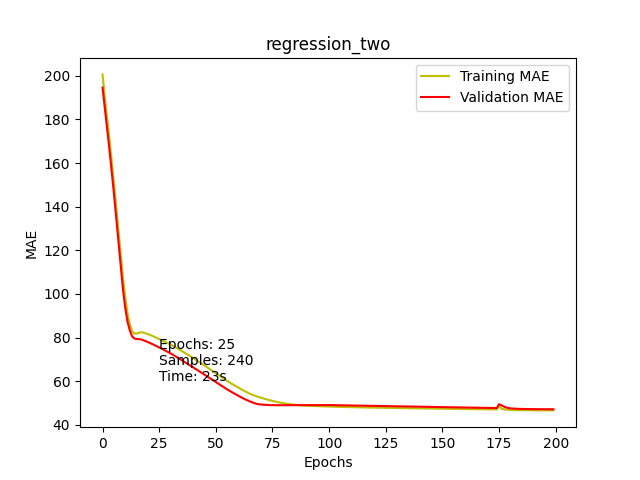
\includegraphics[height=5cm]{../../Plots/ba_plots/regr2/woregr2tr.png}
    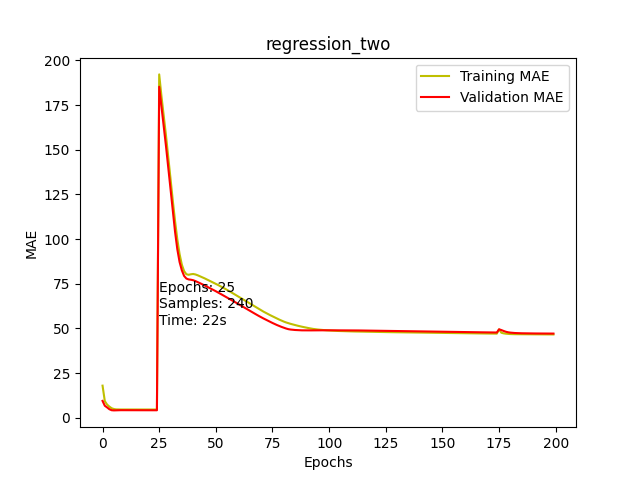
\includegraphics[height=5cm]{../../Plots/ba_plots/regr2/1TFtr.png}
    \caption{\label{fig:regr2tf} 
    \small{In der Abbildung sind links die Ergebnisse des Tests Regr2:240/25 und rechts die des Tests Regr2:TF1/240/25 dargestellt. Der 
    MAE zwischen Trainings- und Validationsset weist dabei kaum Unterschiede auf, was auf ein fehlendes Overfitting 
    hinweist.}}
\end{figure}

Das Overfitting-Problem tritt ausschließlich bei der Klassifikation auf. Dies lässt darauf schließen, dass die Ursache in der verwendeten 
Loss-Funktion oder Aktivierungsfunktion für die Klassifikationsaufgaben liegt.
